\begin{frame}{CNN architecture}
\begin{figure}
    \centering
    \includegraphics[width=0.65\textwidth]{BackUp/Part6/Img/CNN_model.png}
\end{figure}
\end{frame}

\begin{frame}{CNN images size}

\begin{table}[htbp]
    \centering
    \begin{tabular}{lcccc}
    \hline\hline
        $|\eta|$ range & 0 to 1.4 & 1.4 to 1.8 & 1.8 to 2.0 & 2.0 to 2.5 \\
    \hline
        Sampling 1 & 112 & 112 & 84 & 56 \\
        Sampling 2 & 77 & 77 & 77 & 77 \\
        Sampling 3 & 44 & 44 & 44 & 44 \\
    \hline\hline
    \end{tabular}
    \caption{Number of cells in 7$\times$11 EM calorimeter windows.}
\end{table}    
    
\begin{table}[htbp]
    \centering
    \begin{tabular}{lc}
    \hline\hline
        Sampling & Shape \\
    \hline
        Sampling 1 & (56, 2)\\
        Sampling 2 & (7, 11)  \\
        Sampling 3 & (4, 11) \\
    \hline\hline
    \end{tabular}
    \caption{Image shape of 7$\times$11 windows in each sampling in ($\eta$, $\phi$).}
\end{table}
\end{frame}

\begin{frame}{Example of training images}
\begin{figure}
    \centering
    \subfloat{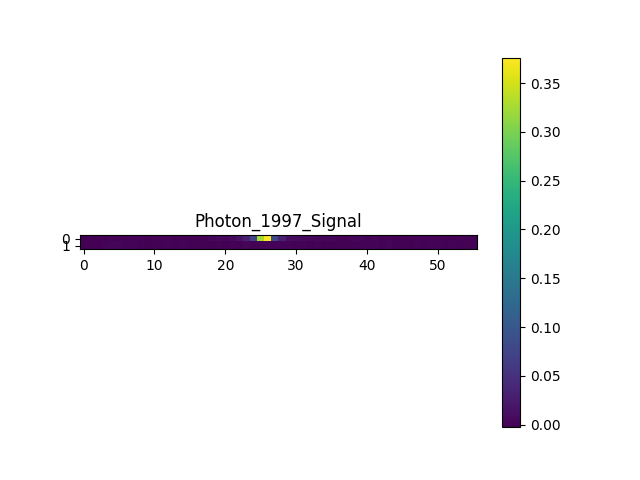
\includegraphics[width=0.32\textwidth]{BackUp/Part6/Img/Sig_Lr1.png}}
    \subfloat{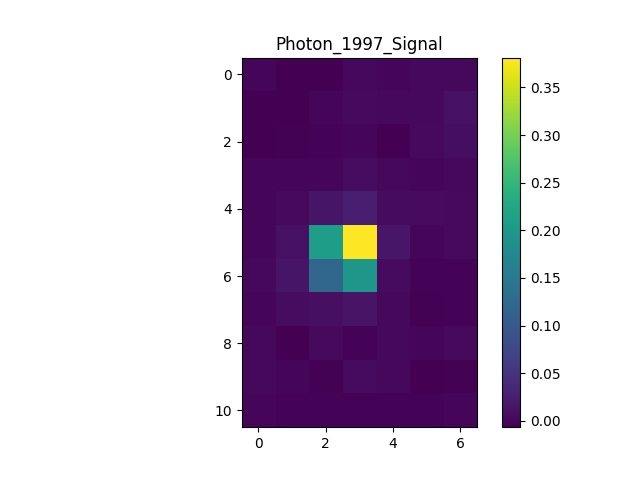
\includegraphics[width=0.32\textwidth]{BackUp/Part6/Img/Sig_Lr2.png}}
    \subfloat{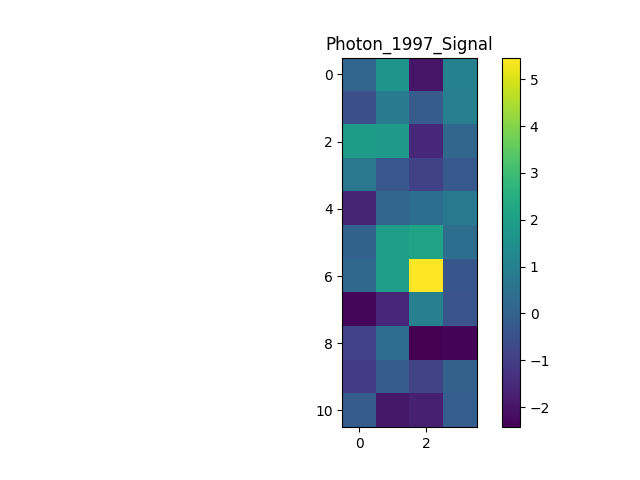
\includegraphics[width=0.32\textwidth]{BackUp/Part6/Img/Sig_Lr3.png}} \\
    \subfloat{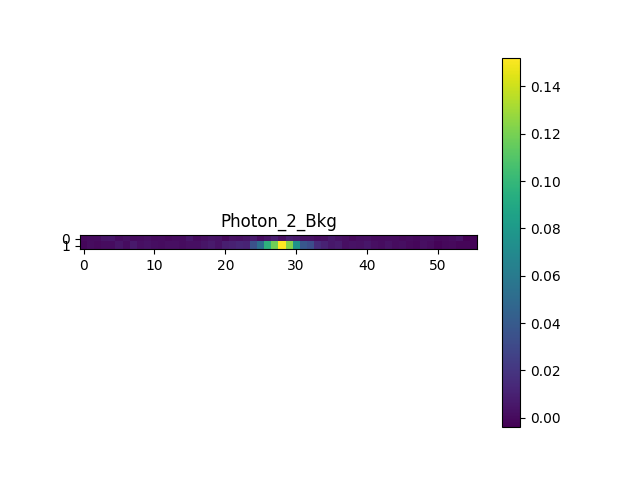
\includegraphics[width=0.32\textwidth]{BackUp/Part6/Img/Bkg_Lr1.png}}
    \subfloat{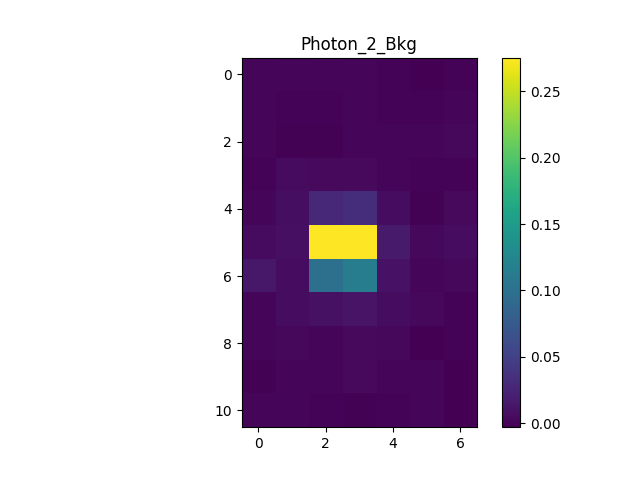
\includegraphics[width=0.32\textwidth]{BackUp/Part6/Img/Bkg_Lr2.png}}
    \subfloat{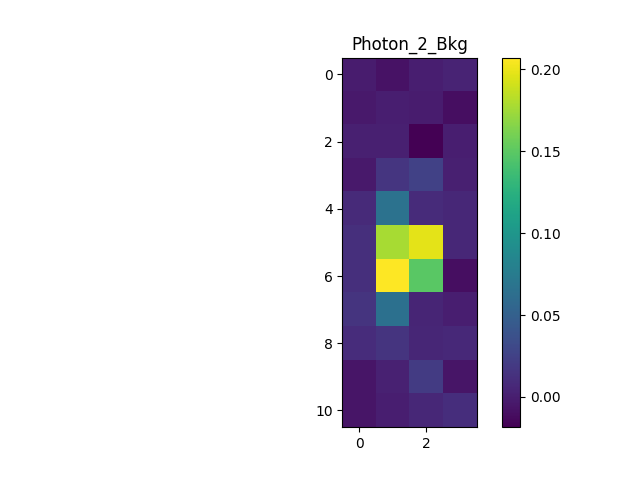
\includegraphics[width=0.32\textwidth]{BackUp/Part6/Img/Bkg_Lr3.png}}
\end{figure}

    
\end{frame}

\begin{frame}{CNN vs DNN for photon identification}
\begin{itemize}
    \item SS-DNN trained on shower shapes variables
    \item CNN trained using images 
\end{itemize}
\begin{figure}
    \centering
    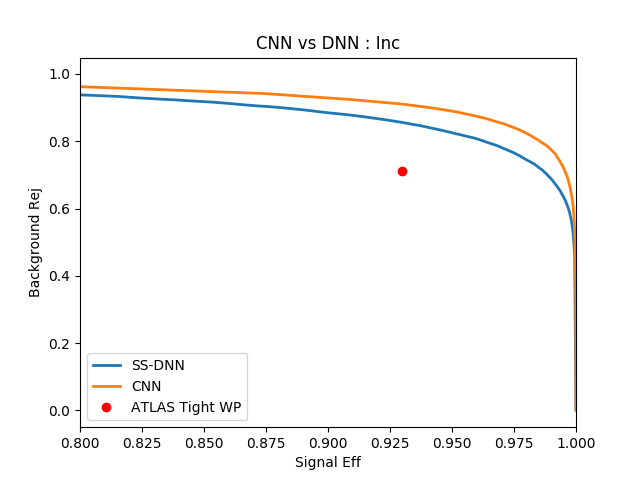
\includegraphics[width=0.6\textwidth]{BackUp/Part6/Img/CNN_vs_DNN.png}
\end{figure}
\end{frame}

\begin{frame}{CNN performance compared to cut-based}
    \begin{figure}
        \centering
        \subfloat{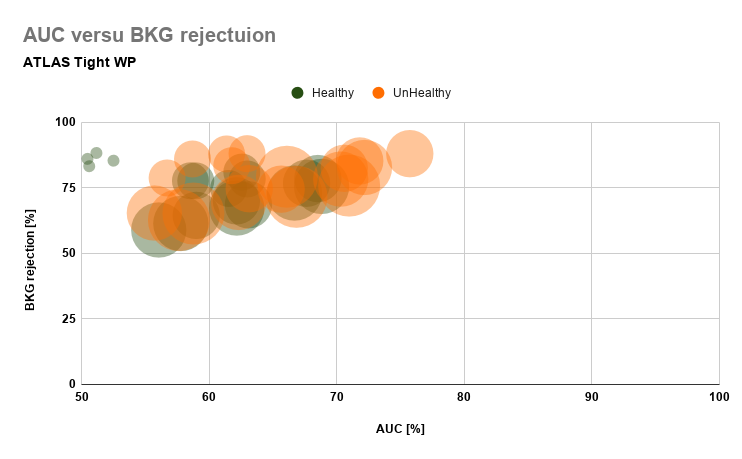
\includegraphics[width=0.5\textwidth]{BackUp/Part6/Img/Tight_auc_vs_eff.png}}
        \subfloat{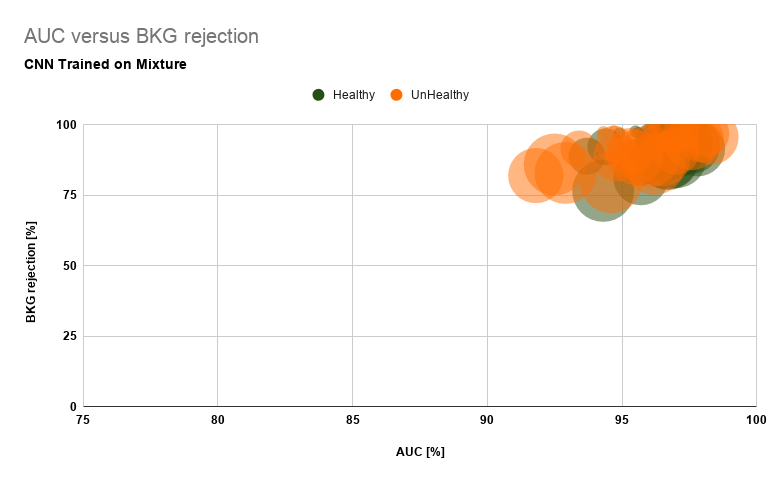
\includegraphics[width=0.5\textwidth]{BackUp/Part6/Img/CNN_auc_vs_eff.png}}
    \end{figure}
\end{frame}

\begin{frame}{CNN signal improvement}
\begin{figure}
    \centering
    \subfloat{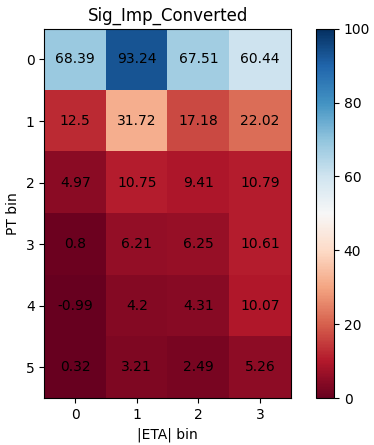
\includegraphics[width=0.4\textwidth]{BackUp/Part6/Img/Sig_Imp_Converted.png}}
    \subfloat{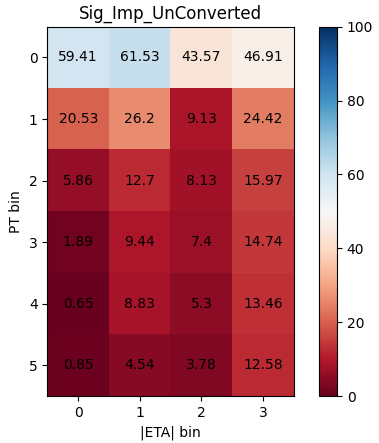
\includegraphics[width=0.4\textwidth]{BackUp/Part6/Img/Sig_Imp_UnConverted.png}}
\end{figure}
$p_T$ = [10, 20, 30, 40, 60, 80, $\infty$], $|\eta|$ = [0, 0.6, 1.37, 1.52, 1.8, 2.4]
\end{frame}

\begin{frame}{CNN background rejection}
    \begin{figure}
        \centering
        \subfloat{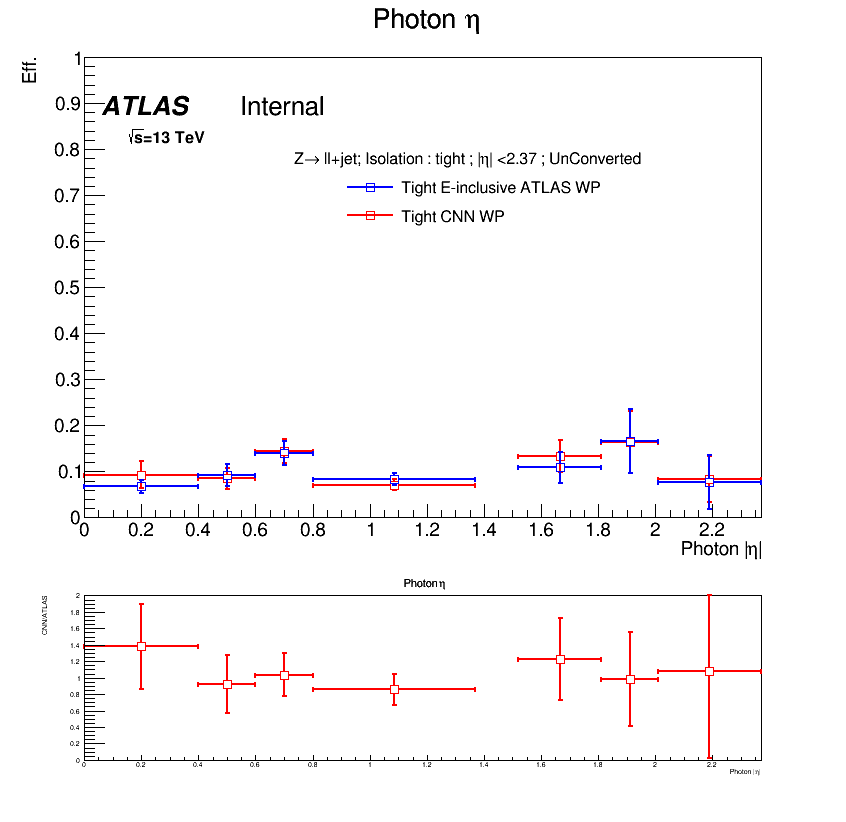
\includegraphics[width=0.5\textwidth]{BackUp/Part6/Img/Bkg_rej_UnConverted.png}}
        \subfloat{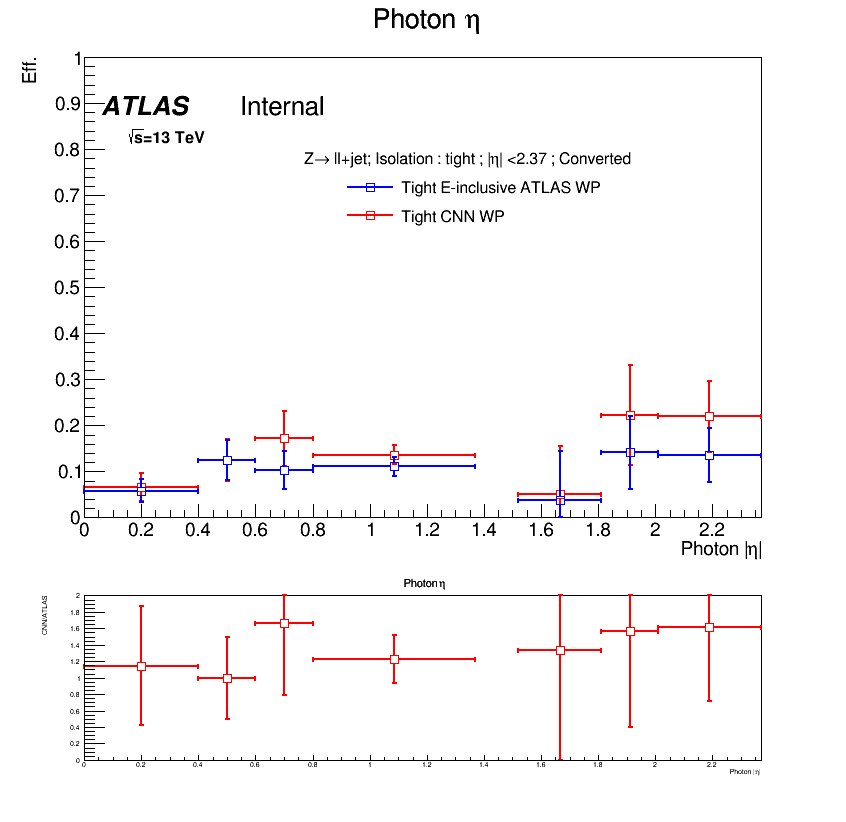
\includegraphics[width=0.5\textwidth]{BackUp/Part6/Img/Bkg_rej_Converted.png}}
    \end{figure}
\end{frame}

\begin{frame}{CNN efficiency, $|\eta| < 0.6$}
    \begin{figure}
        \centering
        \subfloat{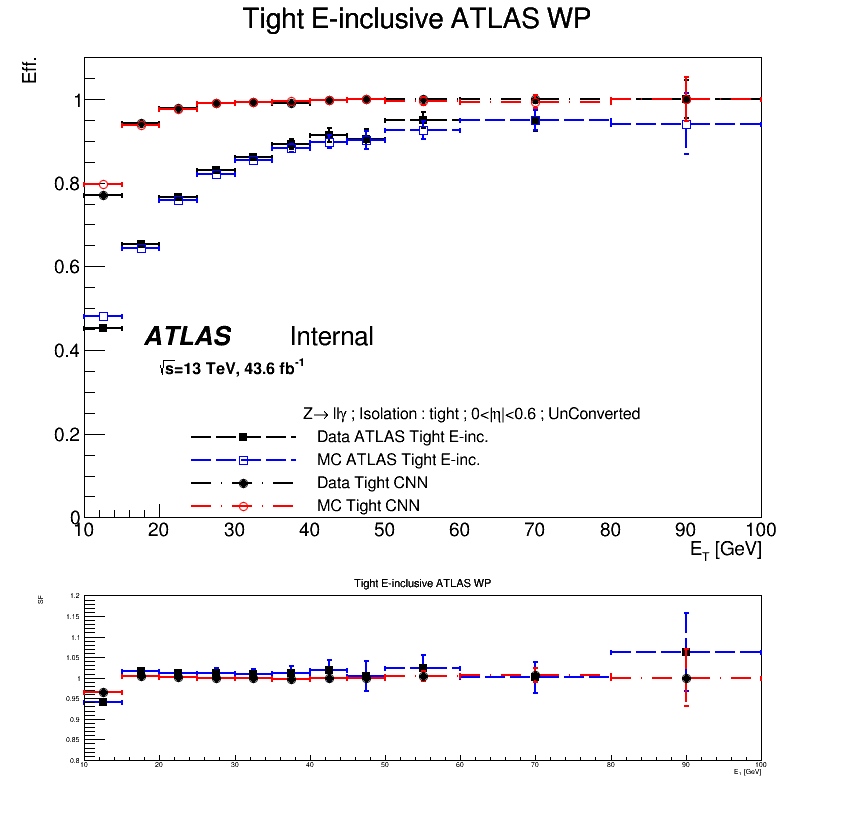
\includegraphics[width=0.5\textwidth]{BackUp/Part6/Img/Tight_Inc_vs_Tight_CNN__UnConverted_Iso_tight_Wgt_ETA_Bin_1.png}}
        \subfloat{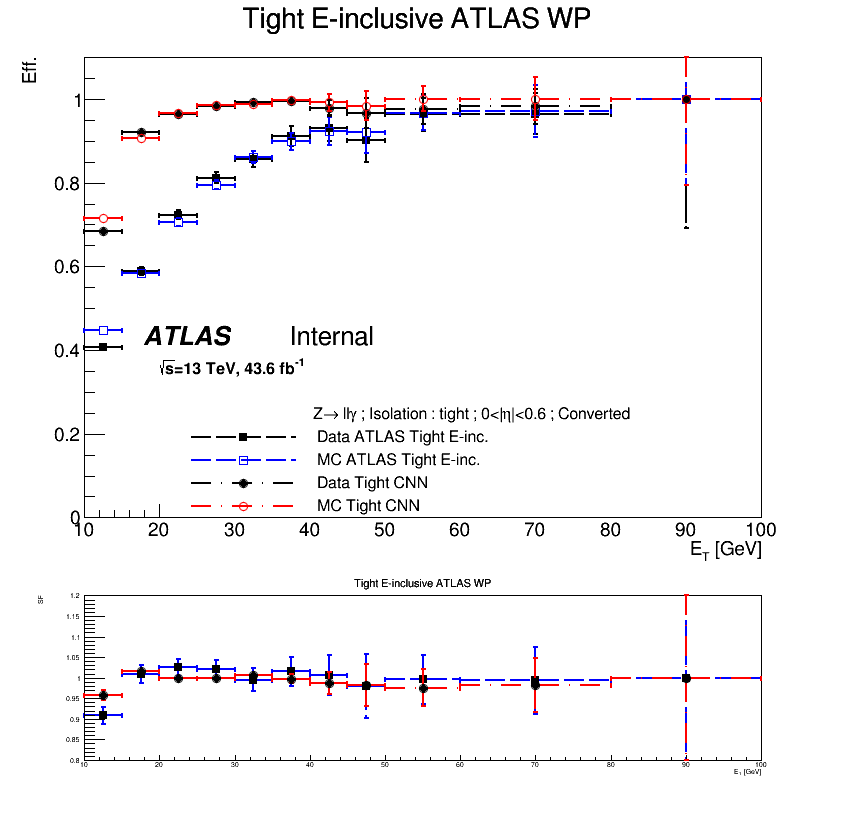
\includegraphics[width=0.5\textwidth]{BackUp/Part6/Img/Tight_Inc_vs_Tight_CNN__Converted_Iso_tight_Wgt_ETA_Bin_1.png}}
    \end{figure}
\end{frame}
\begin{frame}{CNN efficiency, $0.6 < |\eta| < 1.37$}
    \begin{figure}
        \centering
        \subfloat{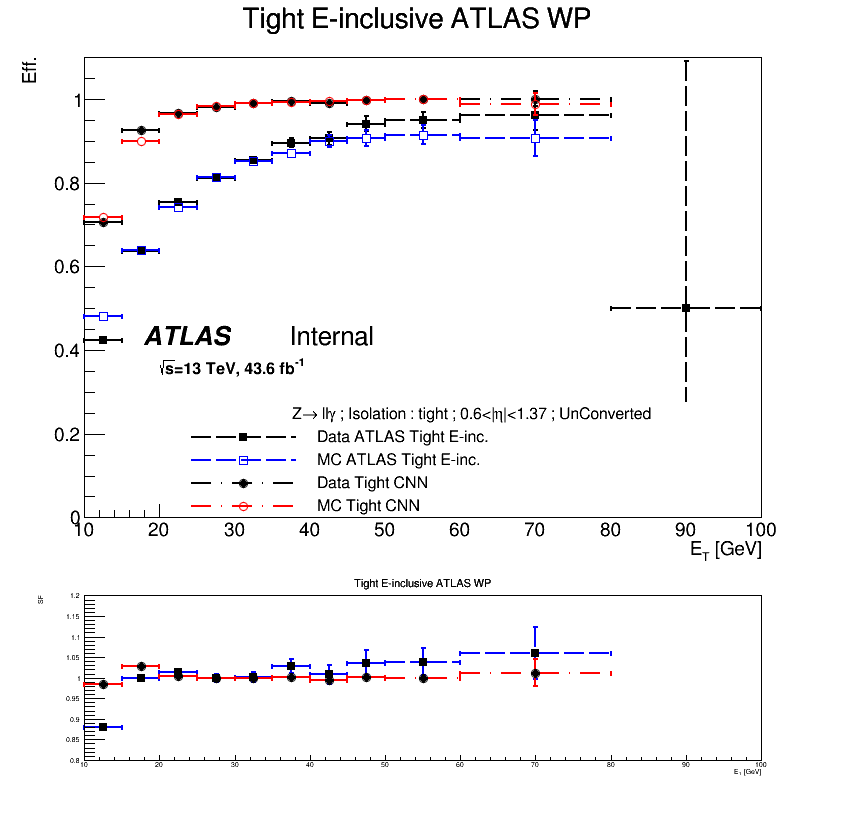
\includegraphics[width=0.5\textwidth]{BackUp/Part6/Img/Tight_Inc_vs_Tight_CNN__UnConverted_Iso_tight_Wgt_ETA_Bin_2.png}}
        \subfloat{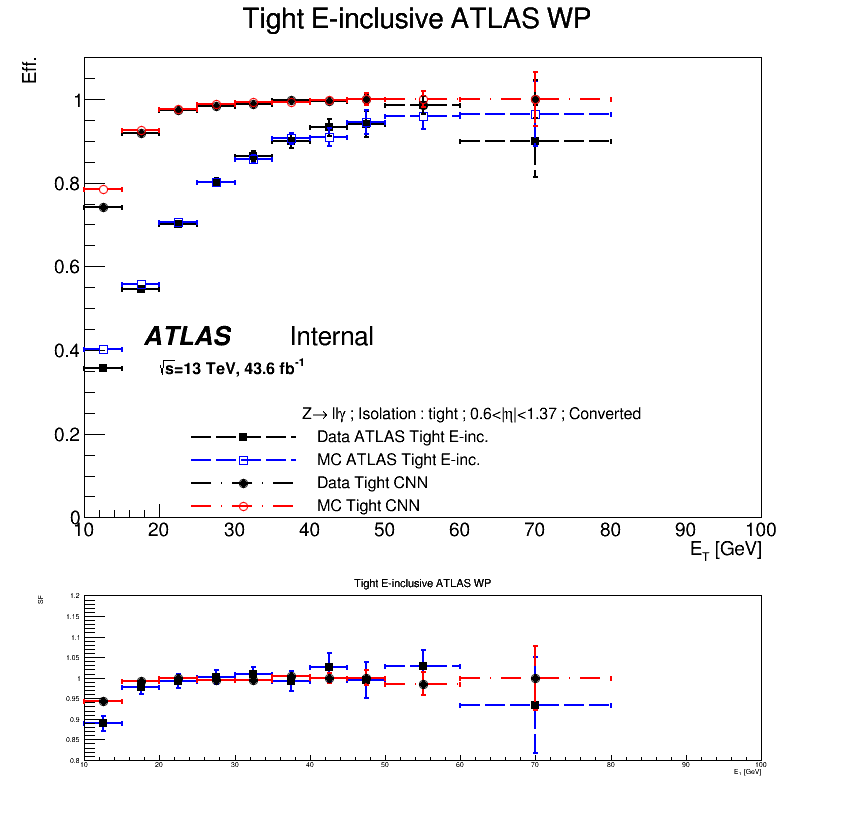
\includegraphics[width=0.5\textwidth]{BackUp/Part6/Img/Tight_Inc_vs_Tight_CNN__Converted_Iso_tight_Wgt_ETA_Bin_2.png}}
    \end{figure}
\end{frame}

\begin{frame}{CNN efficiency, $1.81 < |\eta| < 2.01$}
    \begin{figure}
        \centering
        \subfloat{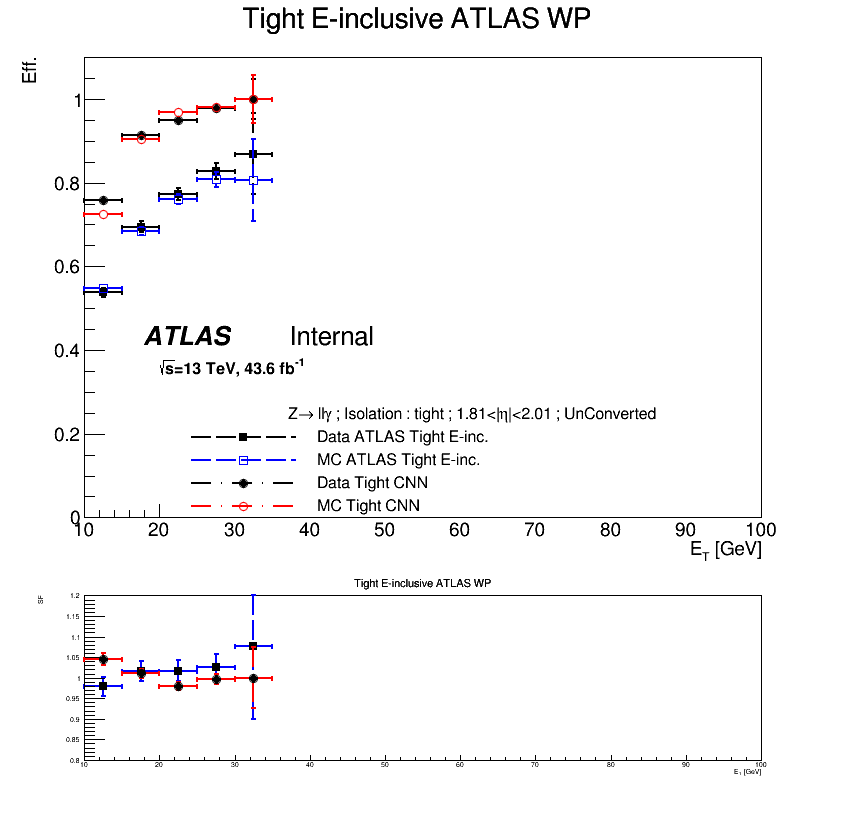
\includegraphics[width=0.5\textwidth]{BackUp/Part6/Img/Tight_Inc_vs_Tight_CNN__UnConverted_Iso_tight_Wgt_ETA_Bin_3.png}}
        \subfloat{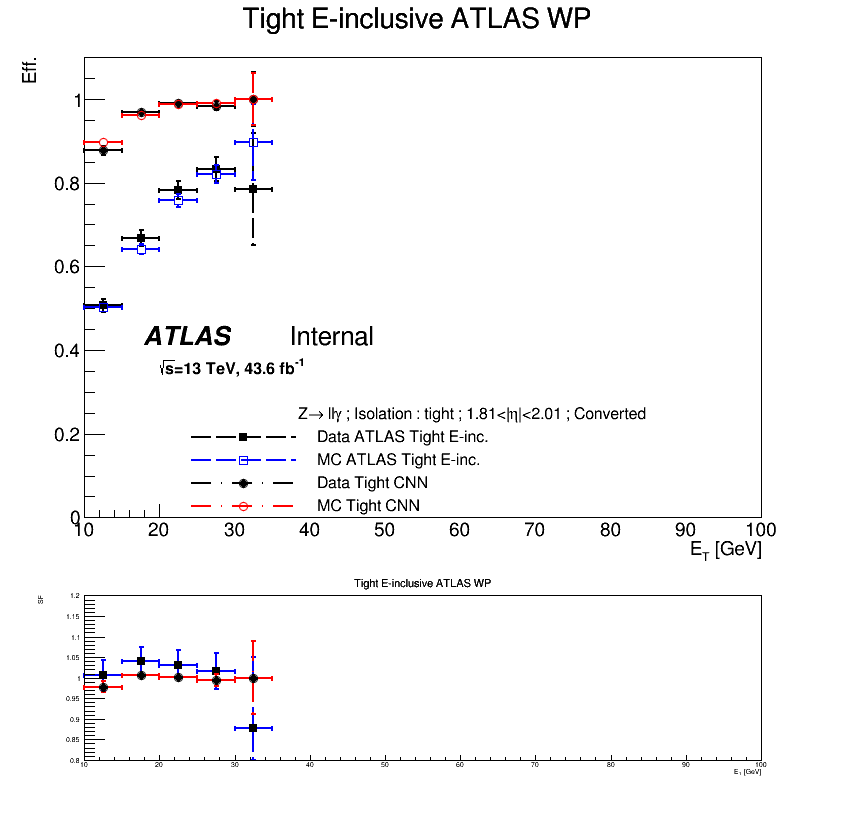
\includegraphics[width=0.5\textwidth]{BackUp/Part6/Img/Tight_Inc_vs_Tight_CNN__Converted_Iso_tight_Wgt_ETA_Bin_3.png}}
    \end{figure}
\end{frame}

\begin{frame}{CNN efficiency, $2.01 < |\eta| < 2.37$}
    \begin{figure}
        \centering
        \subfloat{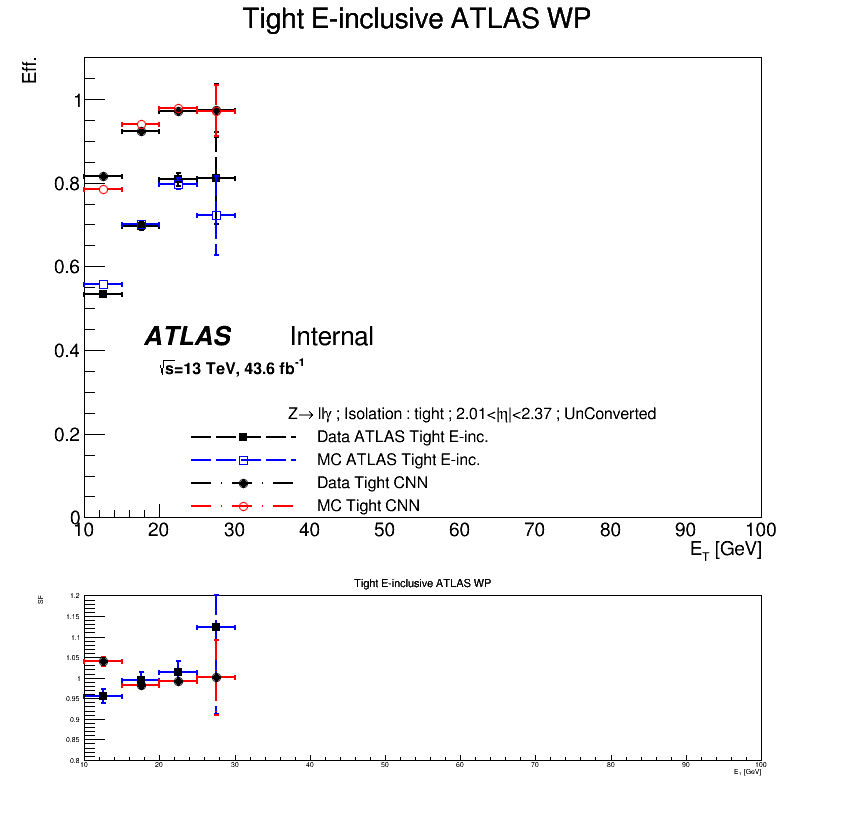
\includegraphics[width=0.5\textwidth]{BackUp/Part6/Img/Tight_Inc_vs_Tight_CNN__UnConverted_Iso_tight_Wgt_ETA_Bin_4.png}}
        \subfloat{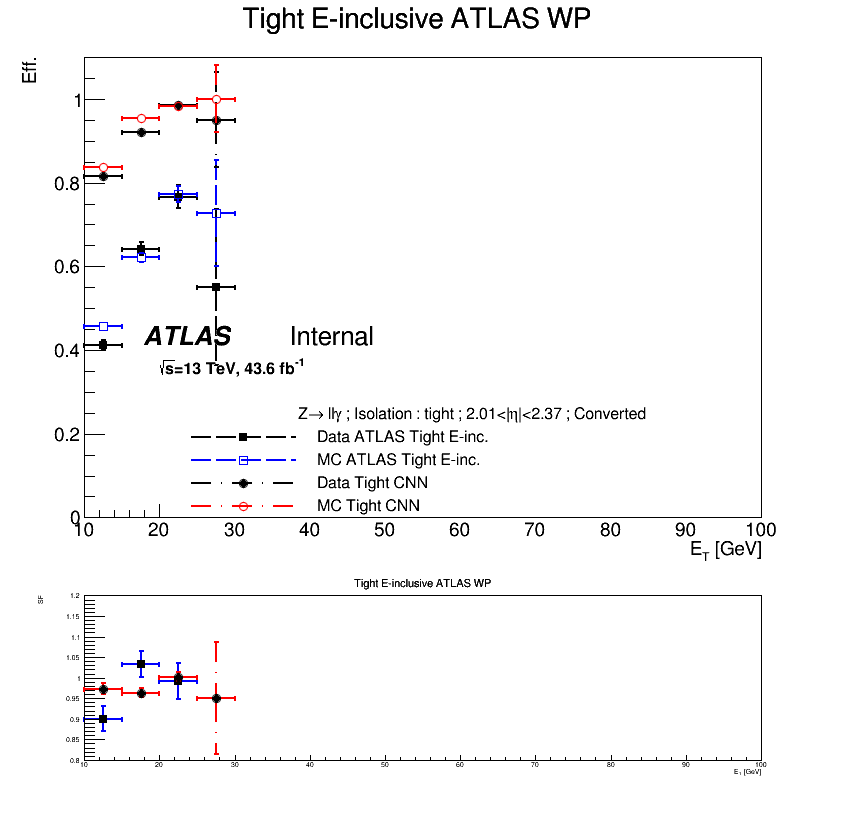
\includegraphics[width=0.5\textwidth]{BackUp/Part6/Img/Tight_Inc_vs_Tight_CNN__Converted_Iso_tight_Wgt_ETA_Bin_4.png}}
    \end{figure}
\end{frame}

\begin{frame}{photon purity before CNN cut}
\begin{table}[htbp]
\centering
\begin{tabular}{lcccccc}
\hline\hline
                             & \multicolumn{3}{c}{Unconverted}               & \multicolumn{3}{c}{Converted}                \\
                            \hline
                             & $ee\gamma$           & $\mu\mu\gamma$           & $ll\gamma$           & $ee\gamma$           &  $\mu\mu\gamma$          & $ll\gamma$           \\
    \hline
10 $ < E_T < $ 15 & 98.1$\pm$4.7   &   96.2$\pm$1.9   &   96.6$\pm$1.8   &   97.8$\pm$7.7   &   95.7$\pm$3.4    &   96.2$\pm$3.1  \\
15 $ < E_T < $ 20 & 99.4$\pm$12.7  &   99.1$\pm$5.1   &   90.7$\pm$1.9   &   99.3$\pm$20.2  &   98.7$\pm$7.5    &   98.8$\pm$6.9  \\
20 $ < E_T < $ 25 & 99.5$\pm$24.2  &   99.6$\pm$10.3  &   99.6$\pm$9.5   &   99.2$\pm$29.4  &   99.4$\pm$13.3   &   99.2$\pm$11.2 \\
25 $ < E_T < $ 30 & 99.4$\pm$33.8  &   99.7$\pm$15.2  &   99.7$\pm$14.5  &   99.3$\pm$51.4  &   99.5$\pm$19.1   &   99.5$\pm$18.2    \\
30 $ < E_T < $ 100 & 99.1$\pm$33   &   99.7$\pm$17.8  &   99.7$\pm$16.5  &   99.1$\pm$50.8  &   99.6$\pm$23.4   &   99.5$\pm$21.4 \\
\hline\hline
\end{tabular}
\caption{Fitted photon purity in \% of all probes, before tight CNN WP. The uncertainties are only statistical.}
\label{tab:gamma:CNN:Zllg:Purity:B}
\end{table}    
\end{frame}

\begin{frame}{photon purity after CNN cut}
\begin{table}[htbp]
\centering
\begin{tabular}{lcccccc}
\hline\hline
                             & \multicolumn{3}{c}{Unconverted}               & \multicolumn{3}{c}{Converted}                \\
                            \hline

%
                             & $ee\gamma$           & $\mu\mu\gamma$           & $ll\gamma$           & $ee\gamma$           &  $\mu\mu\gamma$          & $ll\gamma$           \\
    \hline
10 $ < E_T < $ 15 & 99.6$\pm$11.2    & 98.9$\pm$4.1       & 99.1$\pm$3.8    & 99.3$\pm$16.1    & 98.5$\pm$6.4     & 98.7$\pm$6.02  \\
15 $ < E_T < $ 20 & 99.8$\pm$23.1    & 99.7$\pm$8.9       & 99.7$\pm$8.1    & 99.7$\pm$34.1    & 99.6$\pm$13.2    & 99.6$\pm$12.0 \\
20 $ < E_T < $ 25 & 99.8$\pm$38.1    & 99.8$\pm$15.2      & 99.8$\pm$14.1   & 99.7$\pm$46.6    & 99.6$\pm$17.9    & 99.7$\pm$18.1  \\
25 $ < E_T < $ 30  & 99.7$\pm$49.1   & 99.8$\pm$18.8      & 99.8$\pm$18.5   & 99.6$\pm$66.1    & 99.7$\pm$25.6    & 99.7$\pm$25.    \\
30 $ < E_T < $ 100 & 99.5$\pm$45.6   & 99.8$\pm$21.2      & 99.8$\pm$20.7   & 98.9$\pm$49.4    & 99.7$\pm$28.5    & 99.7$\pm$25.8     \\
\hline\hline
\end{tabular}
\caption{Fitted photon purity in \%  of all probes, after tight CNN WP. The uncertainties are only statistical.}
\label{tab:gamma:CNN:Zllg:Purity:A}
\end{table}
\end{frame}

\begin{frame}{scale factors for unconverted}
\begin{table}[htbp]
    \centering
   \begin{tabular}{lcccc}
   \hline\hline
     & 0 $ < |\eta| < $ 0.6 & 0.6 $ < |\eta| < $ 1.37 & 1.81 $ < |\eta| < $ 2.01  & 2.01 $ < |\eta| < $ 2.37 \\
    \hline
10 $ < E_T < $ 15   & 0.965 $\pm$ 0.0046 & 0.984 $\pm$ 0.0051 & 1.045 $\pm$ 0.0155 & 1.04 $\pm$ 0.011\\
15 $ < E_T < $ 20   & 1.01 $\pm$  0.0032 & 1.03 $\pm$ 0.0036  & 1.01 $\pm$ 0.0114 & 0.982 $\pm$ 0.008 \\
20 $ < E_T < $ 25   & 1.002 $\pm$ 0.0026 & 1.003 $\pm$ 0.003  & 0.980 $\pm$ 0.0099 & 0.992 $\pm$ 0.0093\\
25 $ < E_T < $ 30   & 0.999 $\pm$ 0.0025 & 0.998 $\pm$ 0.003  & 0.997 $\pm$ 0.0114 & 1.001 $\pm$ 0.091\\
30 $ < E_T < $ 35   & 0.999 $\pm$ 0.0032 & 0.999 $\pm$ 0.0032 & 1     $\pm$ 0.0746 & \\
35 $ < E_T < $ 40   & 0.996 $\pm$ 0.0051 & 1.002 $\pm$ 0.0043 &                    & \\
40 $ < E_T < $ 45   & 0.999 $\pm$ 0.0067 & 0.995 $\pm$ 0.0077 &                    & \\
45 $ < E_T < $ 50   & 1     $\pm$ 0.0086 & 1.001 $\pm$ 0.0093 &                    & \\
50 $ < E_T < $ 60   & 1.004 $\pm$ 0.0114 & 1     $\pm$ 0.0097 &                    & \\
60 $ < E_T < $ 80   & 1.006 $\pm$ 0.0179 & 1.012 $\pm$ 0.0326 &                    & \\
80 $ < E_T < $ 100  & 1     $\pm$ 0.07   &                    &                    & \\
\hline\hline
\end{tabular}
\caption{Scale factors for tight CNN WP efficiency measured with unconverted photons from $Z\rightarrow ll\gamma$ decays, in various bins of pseudorapidity and transverse energy. The uncertainty includes only statistical components.}
\end{table}
\end{frame}

\begin{frame}{scale factors for converted}
\begin{table}[htbp]
    \centering
   \begin{tabular}{lcccc}
   \hline\hline
     & 0 $ < |\eta| < $ 0.6 & 0.6 $ < |\eta| < $ 1.37 & 1.81 $ < |\eta| < $ 2.01  & 2.01 $ < |\eta| < $ 2.37 \\
    \hline
10 $ < E_T < $ 15   & 0.96 $\pm$ 0.012   & 0.944 $\pm$ 0.0085 & 0.978 $\pm$ 0.013  & 0.973 $\pm$ 0.013\\
15 $ < E_T < $ 20   & 1.02 $\pm$ 0.008   & 0.99  $\pm$ 0.006  & 1.008 $\pm$ 0.01   & 0.963 $\pm$ 0.011\\
20 $ < E_T < $ 25   & 0.999 $\pm$ 0.0067 & 0.99  $\pm$ 0.0044 & 1.001 $\pm$ 0.008  & 1.003 $\pm$ 0.012\\
25 $ < E_T < $ 30   & 0.999 $\pm$ 0.0063 & 0.995 $\pm$ 0.0044 & 0.994 $\pm$ 0.014  & 0.95  $\pm$ 0.137\\
30 $ < E_T < $ 35   & 1.007 $\pm$ 0.0079 & 0.995 $\pm$ 0.0054 & 1     $\pm$ 0.089  & \\
35 $ < E_T < $ 40   & 0.997 $\pm$ 0.0114 & 1.004 $\pm$ 0.0066 &                    & \\
40 $ < E_T < $ 45   & 0.987 $\pm$ 0.0277 & 0.998 $\pm$ 0.012  &                    & \\
45 $ < E_T < $ 50   & 0.983 $\pm$ 0.0508 & 1.    $\pm$ 0.018  &                    & \\
50 $ < E_T < $ 60   & 0.976 $\pm$ 0.0455 & 0.99  $\pm$ 0.0279 &                    & \\
60 $ < E_T < $ 80   & 0.983 $\pm$ 0.0654 & 1.    $\pm$ 0.078  &                    & \\
80 $ < E_T < $ 100  & 1     $\pm$ 0.37   &                    &                    & \\
\hline\hline
\end{tabular}
\caption{Scale factors for tight CNN WP efficiency measured with converted photons from $Z\rightarrow ll\gamma$ decays, in various bins of pseudorapidity and transverse energy. The uncertainty includes only statistical components.}
\end{table}    
\end{frame}

\begin{frame}{Pile-up effect on CNN}
    \begin{figure}
        \centering
        \subfloat{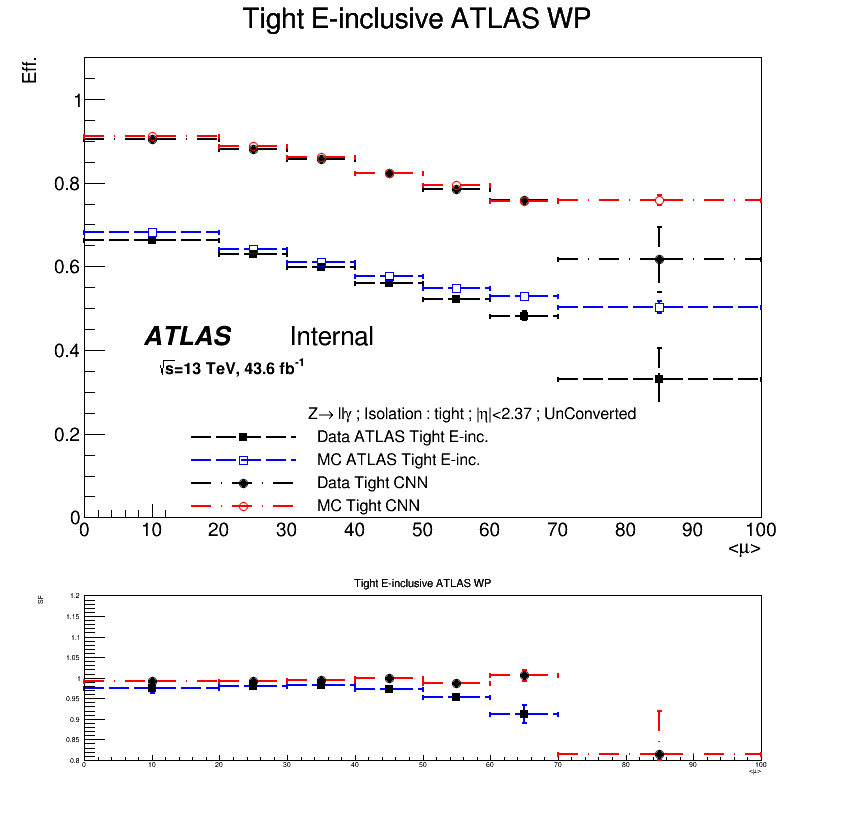
\includegraphics[width=0.5\textwidth]{BackUp/Part6/Img/Tight_Inc_vs_Tight_CNN_mu_UnConverted_Iso_tight_Wgt.png}}
        \subfloat{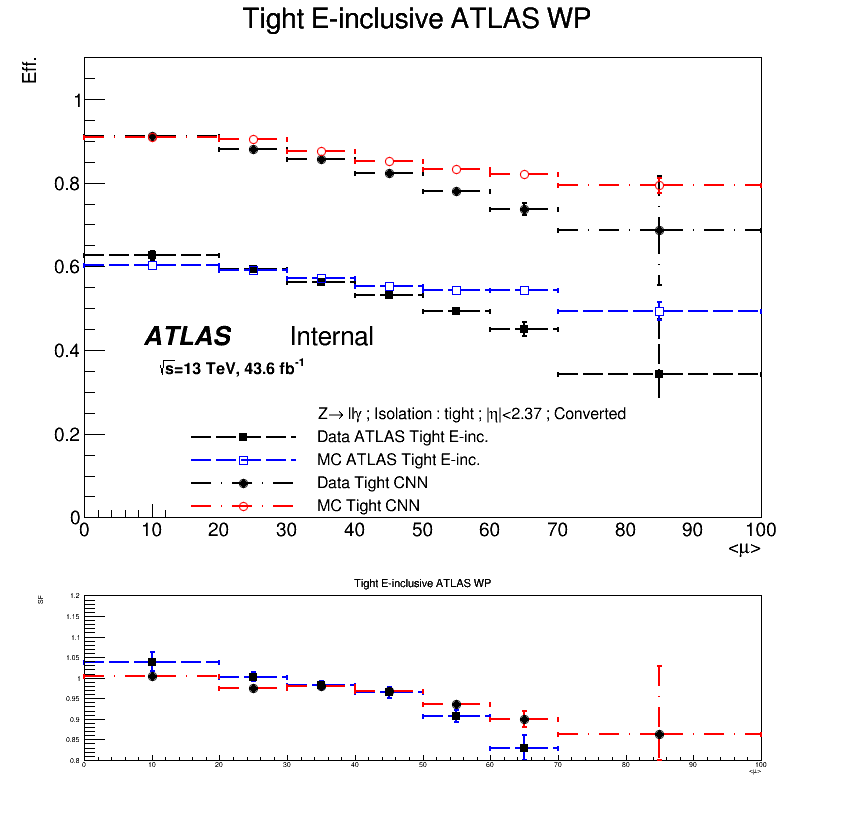
\includegraphics[width=0.5\textwidth]{BackUp/Part6/Img/Tight_Inc_vs_Tight_CNN_mu_Converted_Iso_tight_Wgt.png}}
    \end{figure}
\end{frame}

\begin{frame}{Primary verticies effect on CNN}
    \begin{figure}
        \centering
        \subfloat{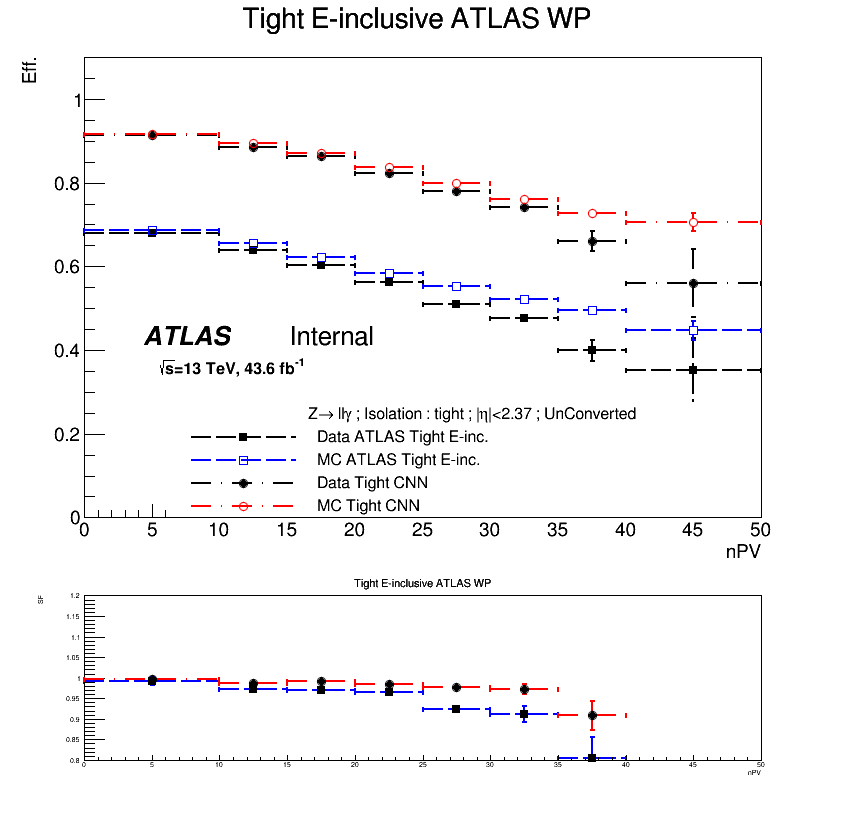
\includegraphics[width=0.5\textwidth]{BackUp/Part6/Img/Tight_Inc_vs_Tight_CNN_MU_UnConverted_Iso_tight_Wgt.png}}
        \subfloat{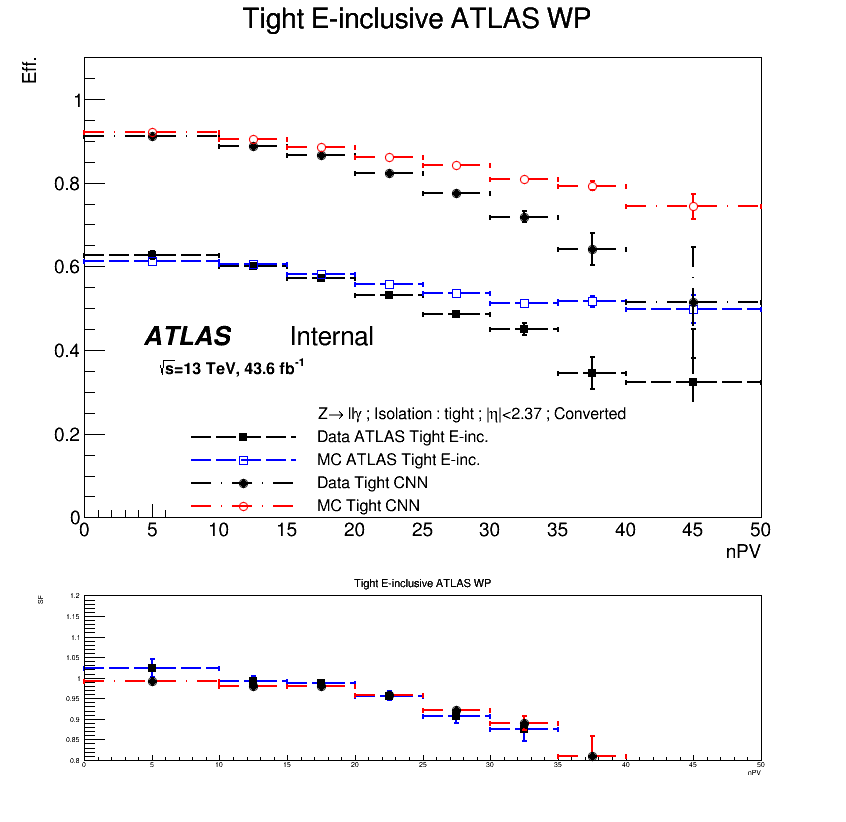
\includegraphics[width=0.5\textwidth]{BackUp/Part6/Img/Tight_Inc_vs_Tight_CNN_MU_Converted_Iso_tight_Wgt.png}}
    \end{figure}
\end{frame}

\begin{frame}{CNN output distribution, $|\eta| < 0.4$}
        \begin{figure}
        \centering
        \subfloat{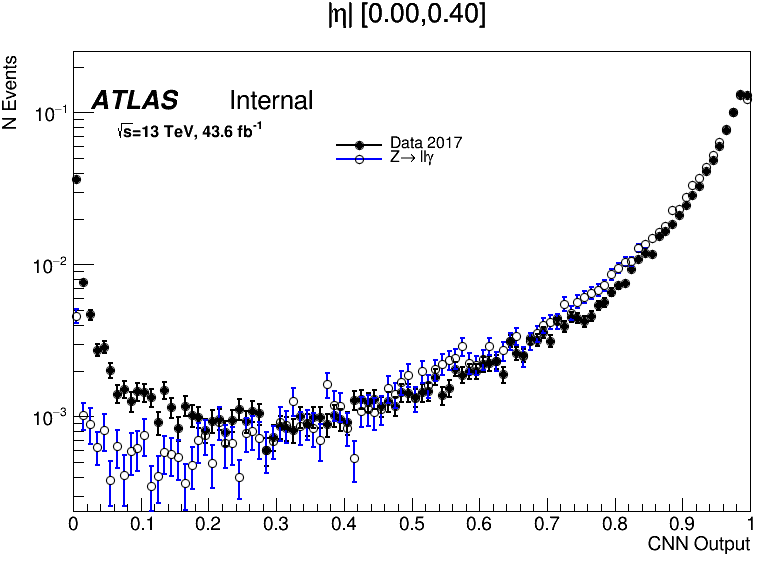
\includegraphics[width=0.5\textwidth]{BackUp/Part6/Img/SubPlot_CNN_output_ETA_bin_0_UnConverted_Iso_tight.png}}
        \subfloat{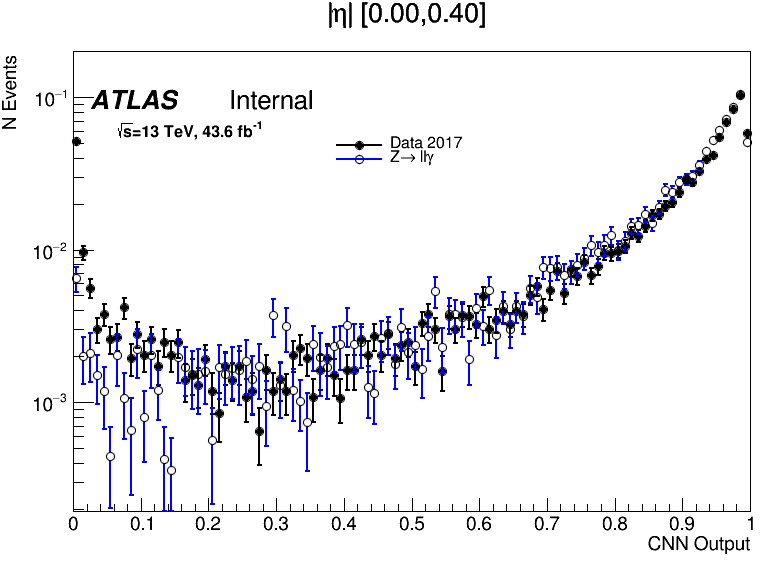
\includegraphics[width=0.5\textwidth]{BackUp/Part6/Img/SubPlot_CNN_output_ETA_bin_0_Converted_Iso_tight.png}}
    \end{figure}
\end{frame}

\begin{frame}{CNN output distribution, $0.4 < |\eta| < 0.6$}
        \begin{figure}
        \centering
        \subfloat{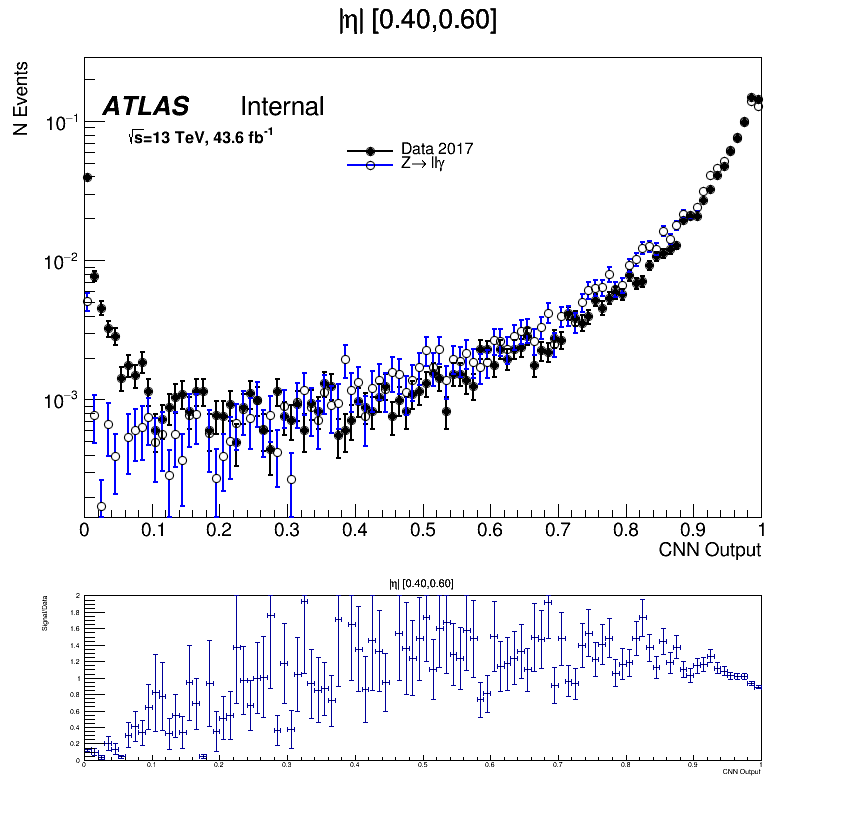
\includegraphics[width=0.5\textwidth]{BackUp/Part6/Img/SubPlot_CNN_output_ETA_bin_1_UnConverted_Iso_tight.png}}
        \subfloat{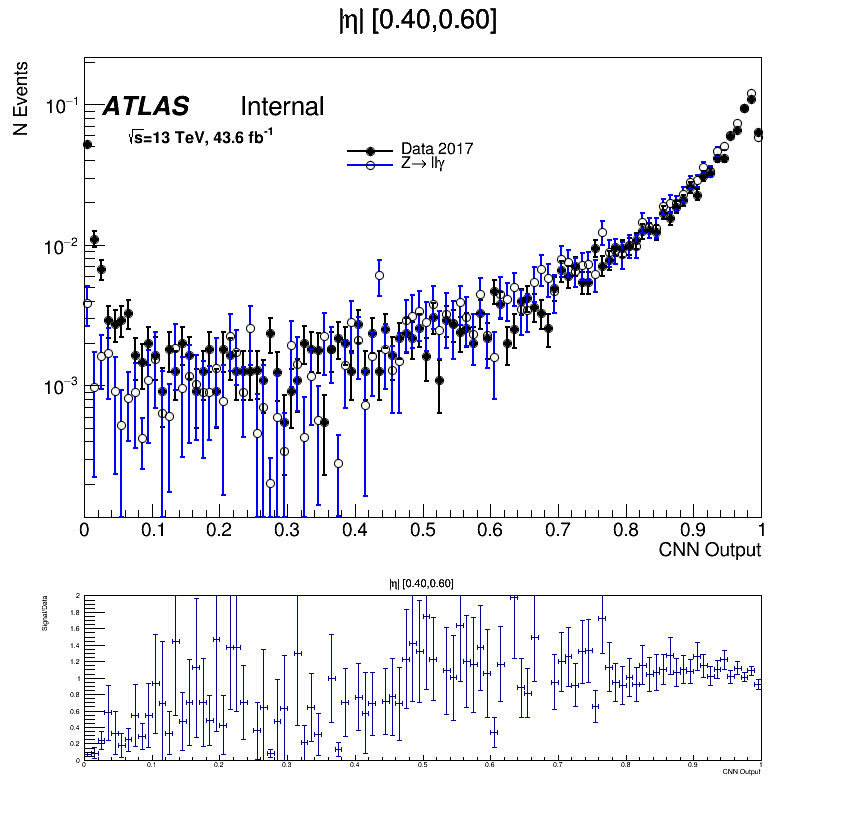
\includegraphics[width=0.5\textwidth]{BackUp/Part6/Img/SubPlot_CNN_output_ETA_bin_1_Converted_Iso_tight.png}}
    \end{figure}
\end{frame}

\begin{frame}{CNN output distribution, $0.6 < |\eta| < 0.8$}
        \begin{figure}
        \centering
        \subfloat{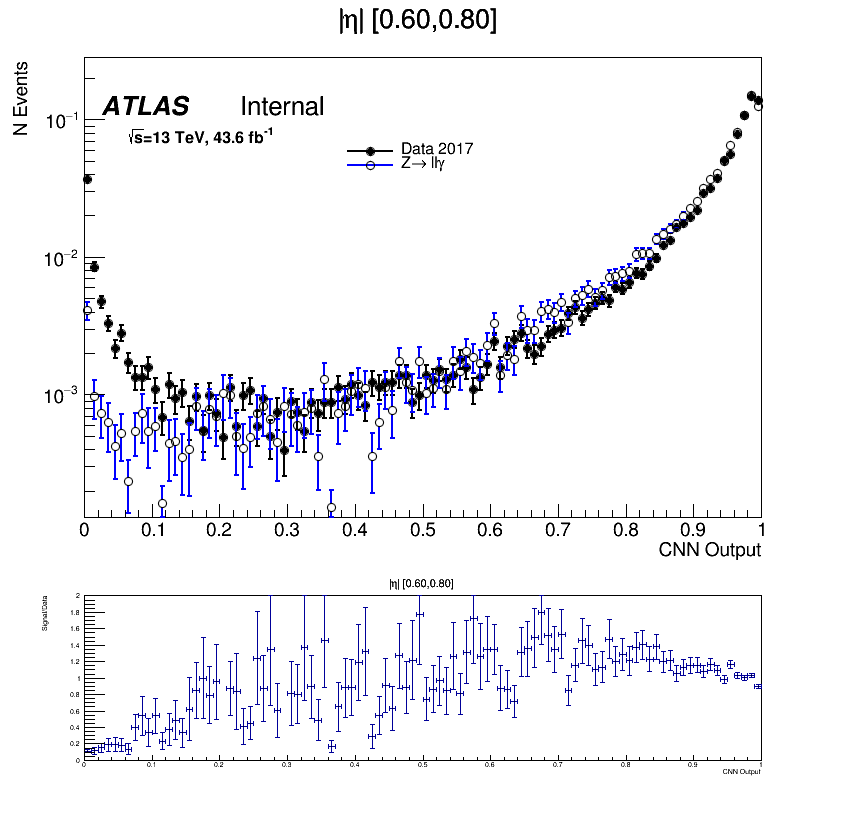
\includegraphics[width=0.5\textwidth]{BackUp/Part6/Img/SubPlot_CNN_output_ETA_bin_2_UnConverted_Iso_tight.png}}
        \subfloat{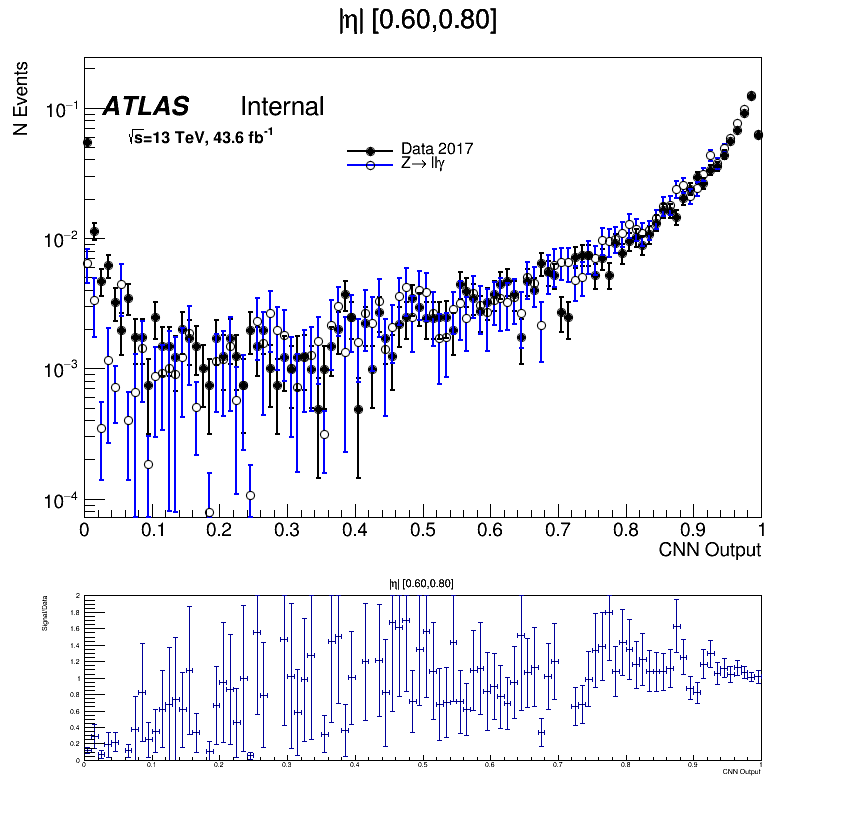
\includegraphics[width=0.5\textwidth]{BackUp/Part6/Img/SubPlot_CNN_output_ETA_bin_2_Converted_Iso_tight.png}}
    \end{figure}
\end{frame}

\begin{frame}{CNN output distribution, $0.6 < |\eta| < 1.37$}
        \begin{figure}
        \centering
        \subfloat{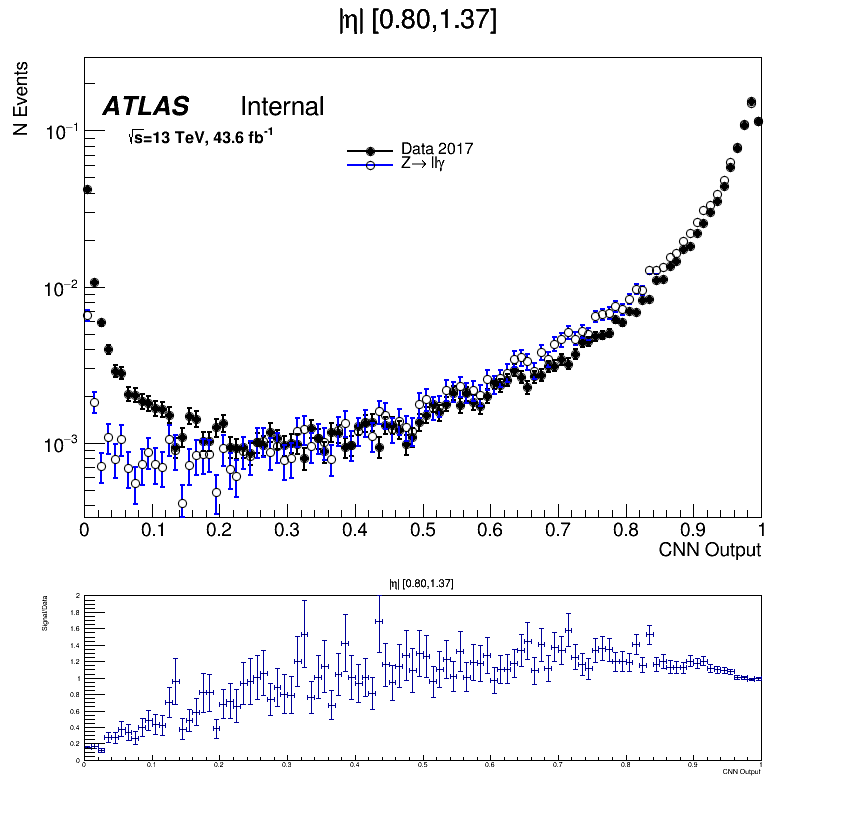
\includegraphics[width=0.5\textwidth]{BackUp/Part6/Img/SubPlot_CNN_output_ETA_bin_3_UnConverted_Iso_tight.png}}
        \subfloat{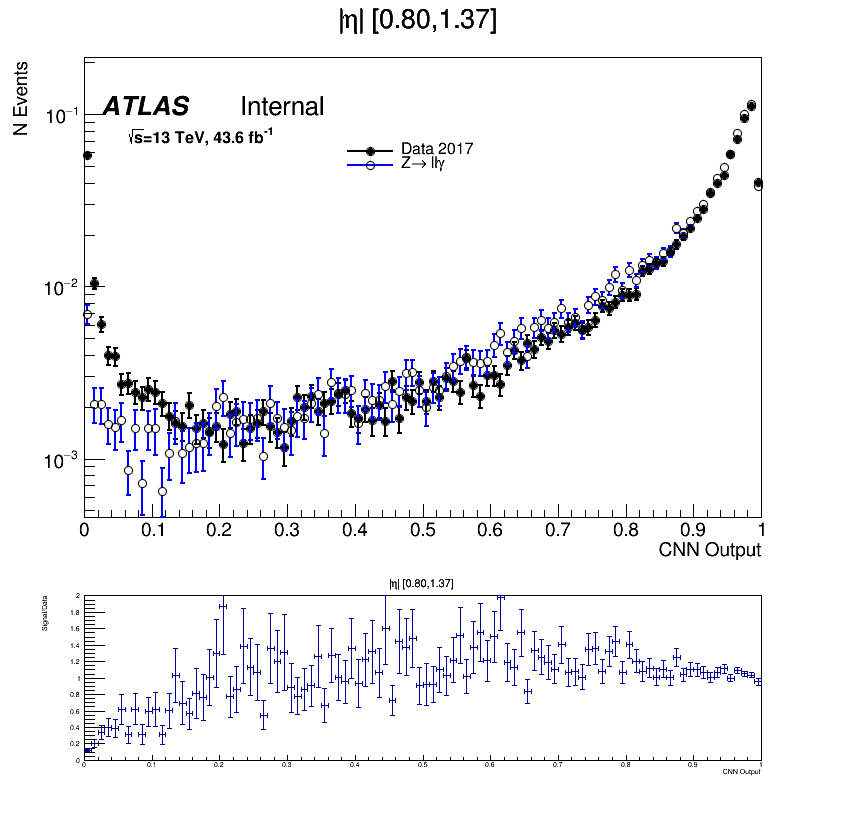
\includegraphics[width=0.5\textwidth]{BackUp/Part6/Img/SubPlot_CNN_output_ETA_bin_3_Converted_Iso_tight.png}}
    \end{figure}
\end{frame}

\begin{frame}{CNN output distribution, $1.52 < |\eta| < 1.81$}
        \begin{figure}
        \centering
        \subfloat{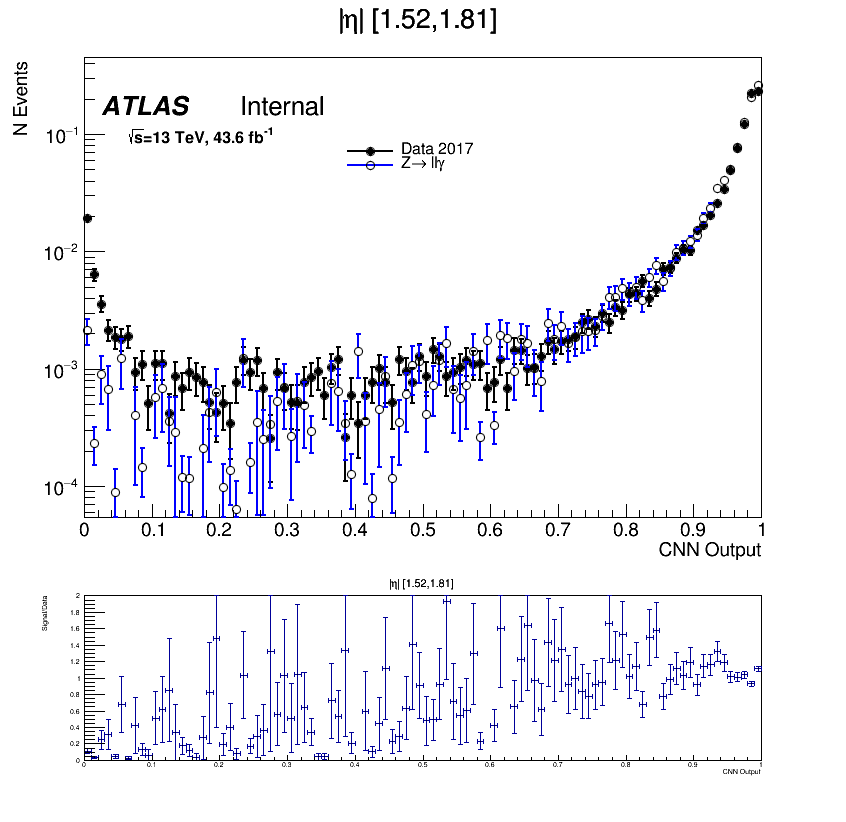
\includegraphics[width=0.5\textwidth]{BackUp/Part6/Img/SubPlot_CNN_output_ETA_bin_5_UnConverted_Iso_tight.png}}
        \subfloat{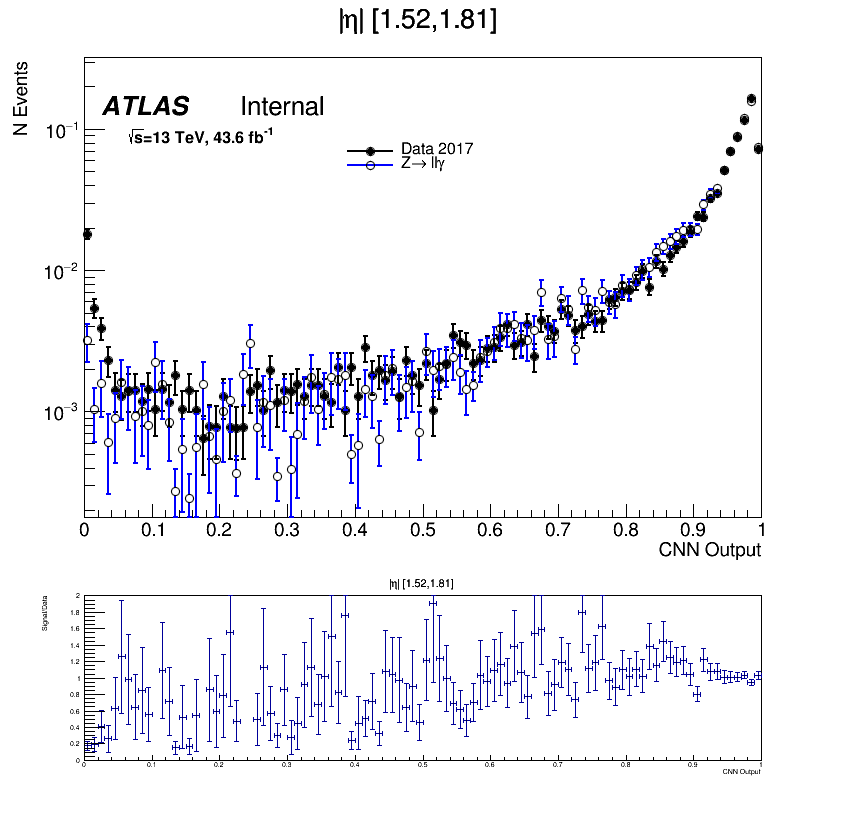
\includegraphics[width=0.5\textwidth]{BackUp/Part6/Img/SubPlot_CNN_output_ETA_bin_5_Converted_Iso_tight.png}}
    \end{figure}
\end{frame}

\begin{frame}{CNN output distribution, $1.81 < |\eta| < 2.01$}
        \begin{figure}
        \centering
        \subfloat{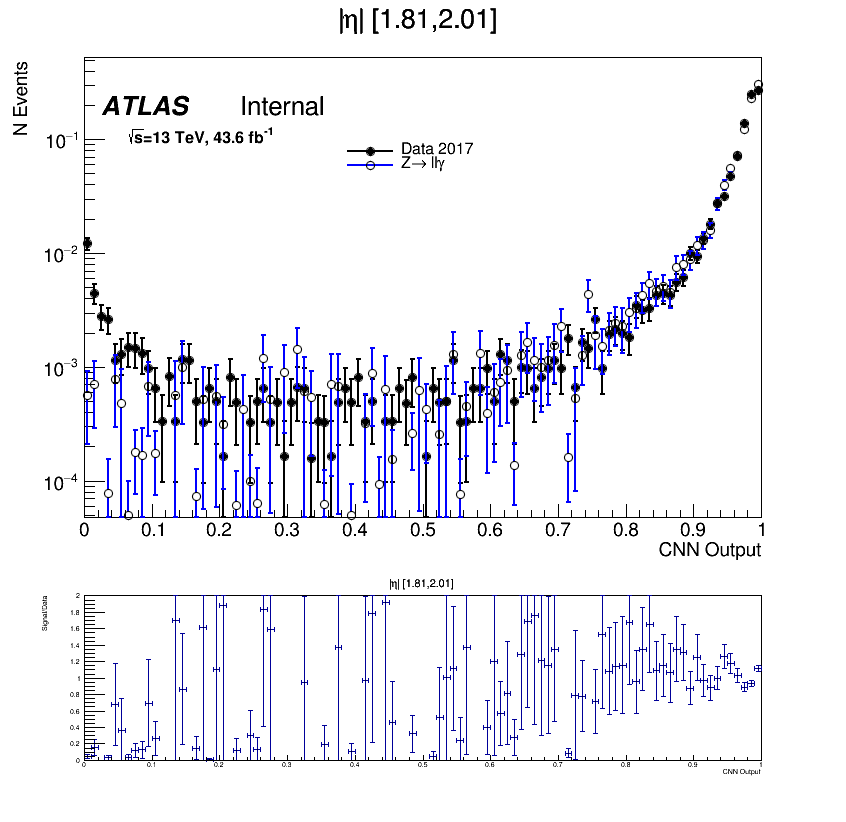
\includegraphics[width=0.5\textwidth]{BackUp/Part6/Img/SubPlot_CNN_output_ETA_bin_6_UnConverted_Iso_tight.png}}
        \subfloat{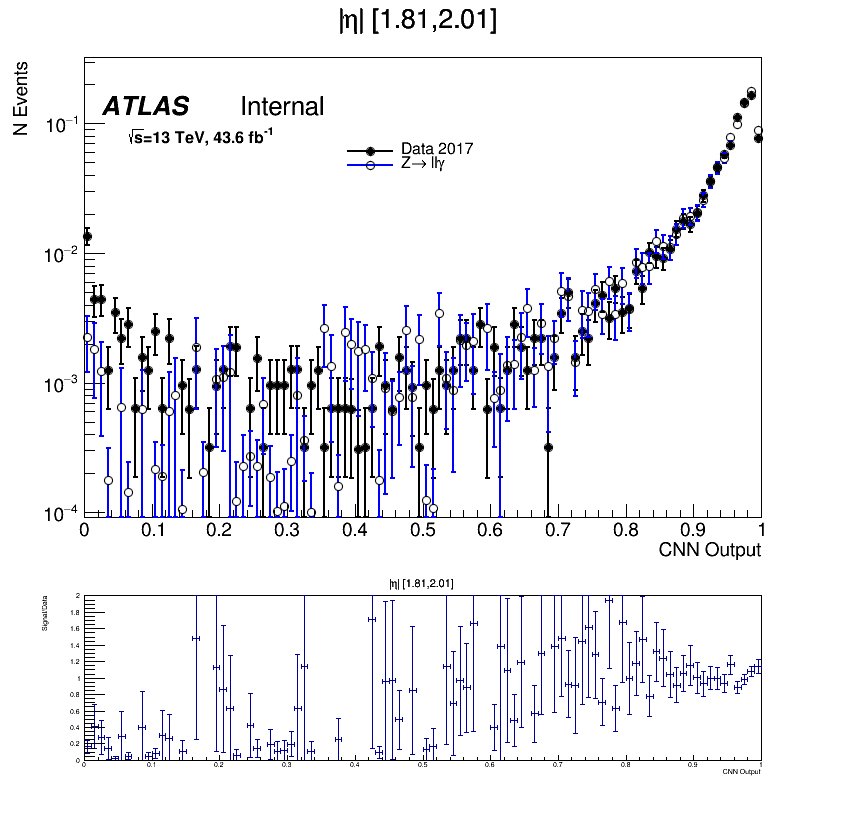
\includegraphics[width=0.5\textwidth]{BackUp/Part6/Img/SubPlot_CNN_output_ETA_bin_6_Converted_Iso_tight.png}}
    \end{figure}
\end{frame}

\begin{frame}{CNN output distribution, $2.01 < |\eta| < 2.37$}
        \begin{figure}
        \centering
        \subfloat{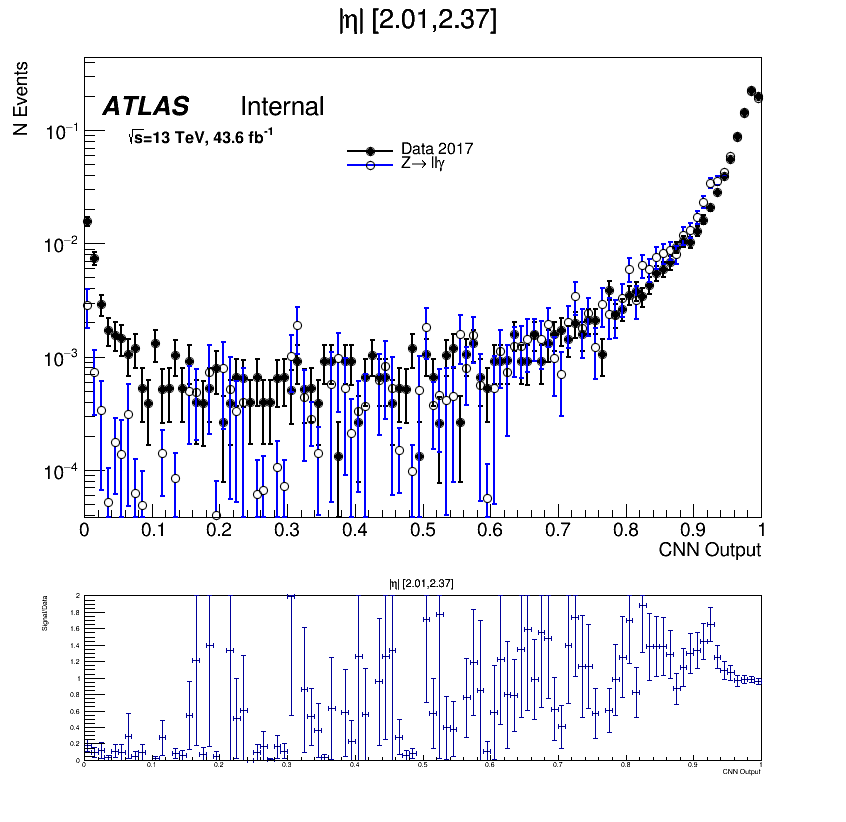
\includegraphics[width=0.5\textwidth]{BackUp/Part6/Img/SubPlot_CNN_output_ETA_bin_7_UnConverted_Iso_tight.png}}
        \subfloat{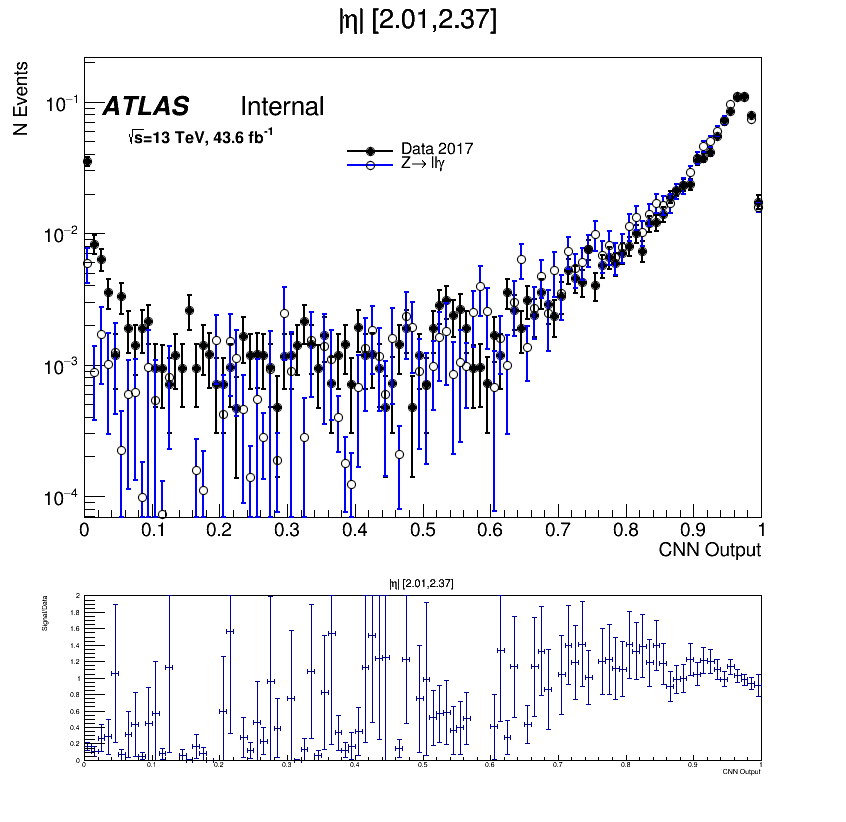
\includegraphics[width=0.5\textwidth]{BackUp/Part6/Img/SubPlot_CNN_output_ETA_bin_7_Converted_Iso_tight.png}}
    \end{figure}
\end{frame}

\begin{frame}{Low efficiency at High $|\eta|$}

\begin{columns}
\column{0.4\textwidth}
\begin{itemize}
    \item CNN performances degrades at low $p_T$ and high $\eta$:
    \begin{itemize}
        \item low energy photons deposit more energy in the first layer.
        \item first layer granularity at high $|\eta|$.
    \end{itemize}
    \item \textbf{Take into account $\eta$ during the training}
\end{itemize}
\column{0.6\textwidth}
    \begin{figure}
        \centering
        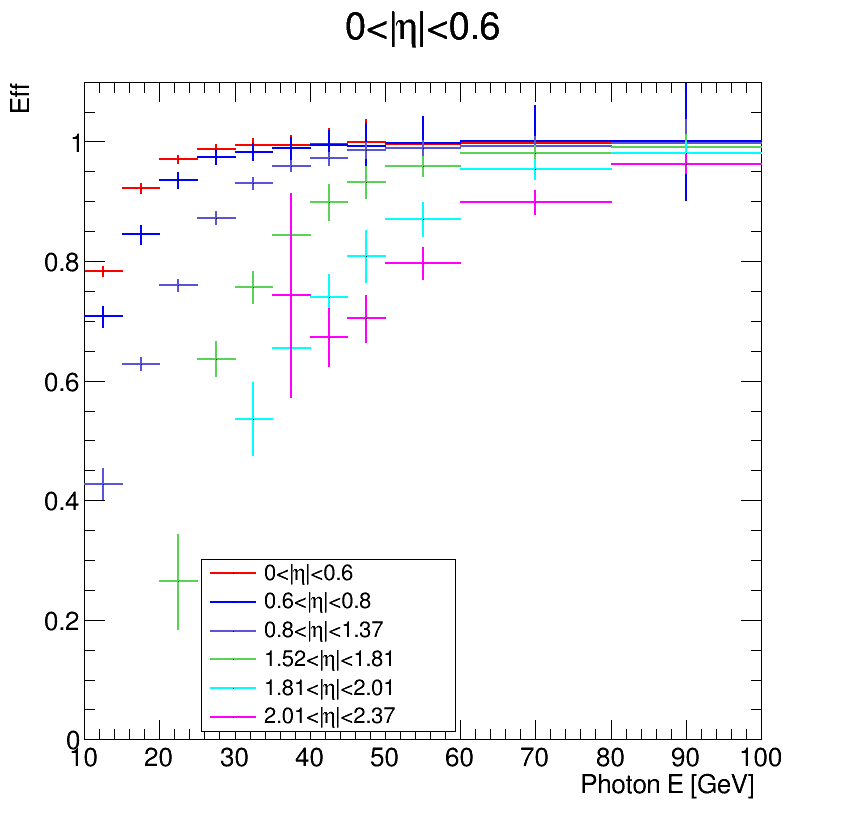
\includegraphics[width=0.9\textwidth]{BackUp/Part6/Img/Eff_vs_Energy.png}
    \end{figure}
\end{columns}
\end{frame}

\begin{frame}{Multi-Task Cascade Convolutional Network (MTCNN)}

\begin{columns}
\column{0.4\textwidth}
\begin{itemize}
    \item Alternative solution for considering photons direction.
    \item Used in face detection.
    \item Can be used with topological clusters.
\end{itemize}

\column{0.6\textwidth}
\begin{figure}
    \centering
    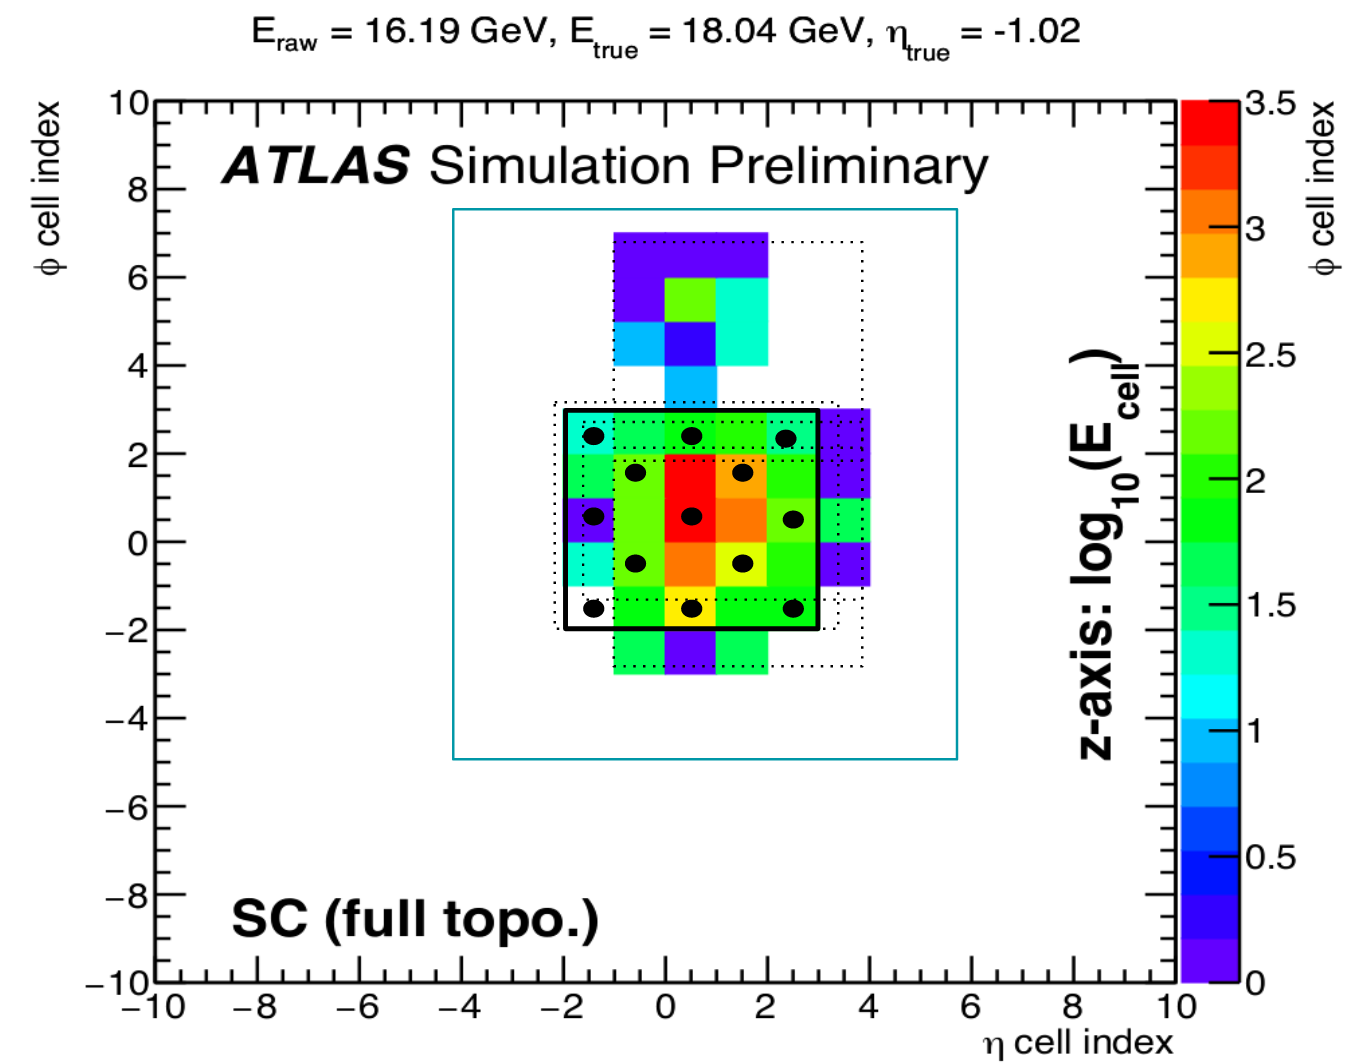
\includegraphics[width=1.\textwidth]{BackUp/Part6/Img/MTCCN.png}
\end{figure}
\end{columns}
\end{frame}

\begin{frame}{Pile-Up Auto-Encoder Denoising}
\begin{columns}
\column{0.4\textwidth}

\begin{itemize}
    \item Efficiency degradation for increasing the Pile-Up (crucial at HL-LHC).
    \item Medicine (image denoising) $\to$ ATLAS (pile-up denoising).
    \item Learn the laten representation of the image using an Auto-Encoder.
\end{itemize}
    
\column{0.6\textwidth}
\begin{figure}
    \centering
    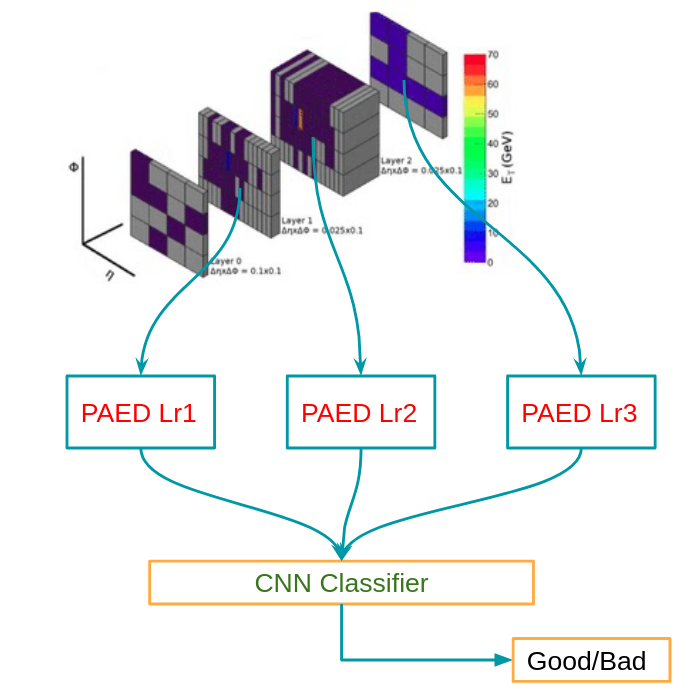
\includegraphics[width=0.8\textwidth]{BackUp/Part6/Img/PAED.png}
\end{figure}
\end{columns}
\end{frame}

\begin{frame}{Cell energy vs Cell energy fraction}
\begin{columns}

\column{0.5\textwidth}
\begin{figure}
    \centering
    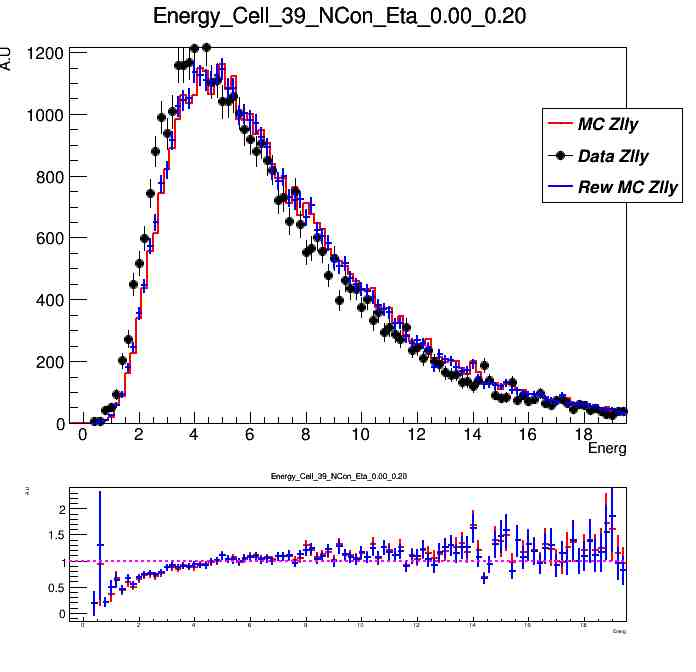
\includegraphics[width=0.8\textwidth]{BackUp/Part6/Img/RewEnergy_Cell_39_NCon_Eta_0.00_0.20Zlly.jpg}
\end{figure}

\column{0.5\textwidth}
\begin{figure}
    \centering
    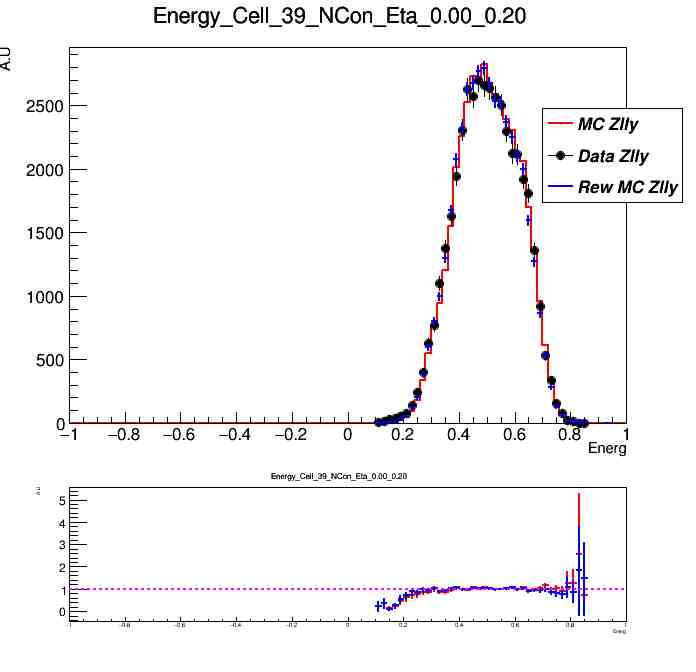
\includegraphics[width=0.8\textwidth]{BackUp/Part6/Img/RewEnergyFrac_Cell_39_NCon_Eta_0.00_0.20Zlly.jpg}
\end{figure}

\end{columns}    
\end{frame}
